\documentclass[a4paper, 10pt, twoside]{article}

\usepackage[top=1in, bottom=1in, left=1in, right=1in]{geometry}
\usepackage[T1]{fontenc}
\usepackage[utf8]{inputenc}
\usepackage[spanish, es-ucroman, es-noquoting]{babel}
\usepackage{setspace}
\usepackage{fancyhdr}
\usepackage{changepage}
\usepackage{lastpage}
\usepackage{amsmath}
\usepackage{amsfonts}
\usepackage{amsthm}
\usepackage{verbatim}
\usepackage{fancyvrb}
\usepackage{graphicx}
\usepackage{float}
\usepackage{enumitem} % Provee macro \setlist
\usepackage{tabularx}
\usepackage{multirow}
\usepackage{hyperref}
\usepackage{xspace}
\usepackage{graphicx}
\usepackage[rightcaption]{sidecap}
\usepackage{ulem} % Provee macro \uwave
\usepackage[toc, page]{appendix}
\usepackage{titlesec}
\usepackage{relsize}
\setcounter{secnumdepth}{4}
\usepackage{multicol}
\usepackage{listings}
\usepackage[usenames,dvipsnames,svgnames,table]{xcolor}

\usepackage{tikz}
\usetikzlibrary{decorations.markings,arrows}

\newcommand{\titulo}{Trabajo Pr\'actico}
\newcommand{\nombre}{Parser de f\'ormulas TeX}
\newcommand{\materia}{Teor\'ia de Lenguajes}
\newcommand{\integrantes}{Mart\'in Fixman}
\newcommand{\cuatrimestre}{Segundo Cuatrimestre de 2015}

\titleformat{\paragraph}
{\normalfont\normalsize\bfseries}{\theparagraph}{1em}{}
\titlespacing*{\paragraph}
{0pt}{3.25ex plus 1ex minus .2ex}{1.5ex plus .2ex}

\pagestyle{fancy}
\thispagestyle{fancy}
\lhead{\titulo}
\rhead{\integrantes}
\renewcommand{\footrulewidth}{0.4pt}
\cfoot{\thepage /\pageref{LastPage}}

\fancypagestyle{caratula} {
   \fancyhf{}
   \cfoot{\thepage /\pageref{LastPage}}
   \renewcommand{\headrulewidth}{0pt}
   \renewcommand{\footrulewidth}{0pt}
}
\raggedbottom

\setlength{\parskip}{0.5em}

\setlist{itemsep=0.5em}

\renewcommand{\appendixtocname}{Apéndices}
\renewcommand{\appendixpagename}{Apéndices}


\lstset{
  backgroundcolor=\color{white},   % choose the background color; you must add \usepackage{color} or \usepackage{xcolor}
  basicstyle=\scriptsize,        % the size of the fonts that are used for the code
  breakatwhitespace=true,         % sets if automatic breaks should only happen at whitespace
  breaklines=true,                 % sets automatic line breaking
  captionpos=b,                    % sets the caption-position to bottom
  commentstyle=\color{Gray},    % comment style
  deletekeywords={...},            % if you want to delete keywords from the given language
  escapeinside={\%*}{*)},          % if you want to add LaTeX within your code
  extendedchars=true,              % lets you use non-ASCII characters; for 8-bits encodings only, does not work with UTF-8
  frame=single,	                   % adds a frame around the code
  keepspaces=true,                 % keeps spaces in text, useful for keeping indentation of code (possibly needs columns=flexible)
  keywordstyle=\color{Blue},       % keyword style
  language=C,                 % the language of the code
  otherkeywords={*,...},           % if you want to add more keywords to the set
  numbers=left,                    % where to put the line-numbers; possible values are (none, left, right)
  numbersep=5pt,                   % how far the line-numbers are from the code
  numberstyle=\tiny\color{gray}, % the style that is used for the line-numbers
  rulecolor=\color{black},         % if not set, the frame-color may be changed on line-breaks within not-black text (e.g. comments (green here))
  showspaces=false,                % show spaces everywhere adding particular underscores; it overrides 'showstringspaces'
  showstringspaces=false,          % underline spaces within strings only
  showtabs=false,                  % show tabs within strings adding particular underscores
  stepnumber=1,                    % the step between two line-numbers. If it's 1, each line will be numbered
  stringstyle=\color{ForestGreen},     % string literal style
  tabsize=2,	                   % sets default tabsize to 2 spaces
  title=\lstname                   % show the filename of files included with \lstinputlisting; also try caption instead of title
}

\begin{document}


\thispagestyle{caratula}

\begin{center}


\includegraphics[height=2cm]{DC.png}
\hfill

\includegraphics[height=2cm]{UBA.jpg}

\vspace{2cm}

Departamento de Computación,\\
Facultad de Ciencias Exactas y Naturales,\\
Universidad de Buenos Aires

\vspace{4cm}

\begin{Huge}
\titulo
\end{Huge}

\vspace{.5cm}

\begin{Huge}
\nombre
\end{Huge}

\vspace{0.5cm}

\begin{Large}
\materia
\end{Large}

\vspace{1cm}

\cuatrimestre

\vspace{4cm}

Mart\'in Fixman

391/11

martinfixman@gmail.com

\end{center}

\newpage

\tableofcontents

\newpage

\section{Introducci\'on}

En este TP debemos parsear una f\'ormula en TeX, que acepte el siguiente lenguaje de entrada

\[
\begin{aligned}
E & \rightarrow & E E & \hspace{3em} & ab \\
& | & E \string^ E & & a^b \\
& | & E \_ E & & a_b \\
& | & E \string^ E \_ E & & a^b_c \\
& | & E \_ E \string^ E & & a_b^c \\
& | & E / E & & \frac{a}{b} \\
& | & ( E ) & & (a) \\
& | & { E } & & a \\
& | & l & & l
\end{aligned}
\]

Y que devuelva un archivo \texttt{svg} equivalente a cierta f\'ormula dada.

\section{Lenguaje de entrada}

Es f\'acil ver que el lenguaje de entrada es ambiguo. Por ejemplo, la f\'ormula de entrada \(a \string^ b / c \_ d\) podr\'ia parsearse equivalentemente como alguna de las siguientes f\'ormulas:

\begin{multicols}{4}
\[ \mathlarger{ a^{\frac{b}{c_d}} } \] \break
\[ \mathlarger{ \frac{a^b}{c_d} } \] \break
\[ \mathlarger{ a^{\frac{b}{c}}_d } \] \break
\[ \mathlarger{ \frac{a^b}{c}_d } \]
\end{multicols}

Para resolver la ambig\"uedad se definen reglas de precedencia a los operadores, a la concatenaci\'on y a la divisi\'on como asociativos a la izquierda, y se hace il\'icito usar el super\'indice y el sub\'indice en varias expresiones sin agrupar. De esa manera, creamos la siguiente gram\'atica, que es equivalente a la gram\'atica anterior pero con las nueva reglas y sin ambig\"uedad:

\[
\begin{aligned}
E & \rightarrow & F / E \\
& | & F \\
F & \rightarrow & G F \\
& | & G \\
G & \rightarrow & H \string^ H \\
& | & H \_ H \\
& | & H \string^ H \_ H \\
& | & H \_ H \string^ H \\
H & \rightarrow & ( E ) \\
& | & { E } \\
& | & l
\end{aligned}
\]

\newpage

\section{Programas usados}

Para parsear las formulas usamos \texttt{flex}, una implementaci\'on de c\'odigo abierto de \texttt{lex}, como un \textbf{tokenizer} que define como se toma cada elemento de la entrada\footnote{En el archivo \texttt{formula.l}}, y \texttt{bison}, una implementaci\'on de c\'odigo abierto de \texttt{yacc}, un \textbf{parser LALR} con gram\'atica anal\'itica para imprimir el resultado\footnote{En el archivo \texttt{formula.y}}.

Una vez que se parsean los archivos, se crea un ejecutable desde el c\'odigo fuente de \texttt{C} resultante usando \texttt{gcc}\footnote{El \texttt{Makefile} se ocupa de procesar todos los fuentes autom\'aticamente}.

El programa se prob\'o usando \texttt{lex 2.6.0}, \texttt{GNU bison 3.0.4}, y \texttt{gcc 5.3.0}, aunque puede andar en otras versiones de los programas. En particular, el Makefile asume que la versi\'on actual de \texttt{gcc} admite \texttt{C11}, aunque puede ser modificado simplemente si la versi\'on en la computadora local no lo hace. La salida fue probada en \texttt{Mozilla Firefox 42.0}, aunque tambi\'en funciona perfectamente en \texttt{Chromium 47.0.2526.80}, la versi\'on de c\'odigo abierto de \texttt{Google Chrome}.

\section{Gram\'atica de atributos}

A pesar de que la gram\'atica usada es relativamente simple, se usa una gram\'atica de atributos m\'as complicada para lograr escribir la salida.

La gram\'atica crea un \'arbol de parseo con las siguientes propiedades:

\begin{itemize}
\item Cada f\'ormula se define como un \'arbol, donde cada nodo corresponde a una operaci\'on, y sus hijos a los elementos en los que se le aplica.
\item El \'arbol es un \'arbol binario no necesariamente completo. Eso significa que cada nodo tiene \(2\), \(1\), \'o \(0\) hijos.
\item Se definen \(5\) operaciones diferentes:
	\begin{description}
		\item[Literal] que siempre es una hoja y corresponde a un literal que se debe imprimir.
		\item[Concat] que siempre tiene dos hijos y corresponde a la concatenaci\'on de dos elementos.
		\item[Caretunder] que tiene uno o dos hijos y corresponde a la operaci\'on de potenciaci\'on y sub\'indice. Notar que las cuatro operaciones correspondientes al noterminal \(G\) pueden ser definidas con esta operaci\'on, y que su padre siempre debe ser \textbf{Concat}. Por ejemplo, \(a^b\) corresponde a \texttt{Concat(Literal('a'), Caretunder(Literal('b'), NULL))}.
		\item[Parentheses] que tiene un solo hijo y represente un par de parentesis entre la f\'ormula representada por este.
		\item[Division] que siempre tiene dos hijos y representa una divisi\'on entre estos.
	\end{description}
\end{itemize}

El parser genera el \'arbol de las hojas hacia la ra\'iz usando una gram\'atica \textbf{LALR} y hace dos operaciones diferentes.

Primero, calcula el tama\~no\footnote{Definido como la tupla <ancho, altura sobre l\'linea, altura bajo l\'inea>} que ocupa la f\'ormula representada por cada nodo de la ra\'iz hacia las hojas (lo que le permite usar el tama\~no de sus hijos como argumento), y devuelve estos m\'as el tama\~no del nodo ra\'iz que es igual al tama\~no total de la im\'agen.

Luego, imprime cada nodo, que significa imprimir el caracter correspondiente si corresponde a un \textbf{Literal}, o imprimir a sus hijos con cierta transformaci\'on que depende de la operaci\'on representada por este nodo. En el caso de \textbf{Parentheses} y \textbf{Division}, se dibujan los parentesis y la linea de la divisi\'on.

\section{Lenguaje de salida}

El objetivo del trabajo es devolver la f\'ormula en un archivo \texttt{svg}. Hay cientos de maneras diferentes de hacer esto, pero por simplicidad el parser devuelve una im\'agen con los siguientes tags:

\begin{description}
\item [<svg>] Indica que lo que est\'a adentro debe parsearse como una imagen \texttt{svg}.
\item [<g>] Abre un bloque gen\'erico en el que se pueden agregar cualquier otro elemento, y se puede cambiar de escala o mover usando los argumentos \texttt{scale} y \texttt{translate}. Se usa en todas las operaciones excepto  \textbf{Literal} para aclarar como se va a modificar cada elemento.
\item [<text>] Imprime cierto texto. Se usa sin ning\'un argumento en \textbf{Literal} para imprimir el literal correspondiente, y en \textbf{Parentheses} para imprimir los parentesis con argumentos que modifican su altura y su posici\'on.
\item [<line>] Imprime una linea recta. Se usa en para imprimir la linea de la divisi\'on en \textbf{Division}\footnote{Tambi\'en fue usado para crear peque\~nas lineas de colores en cada elemento y poder debuguear m\'as facilmente el c\'digo}.
\end{description}

\section{Complicaciones varias}

Adem\'as de algunas ya incluidas, haciendo esta gram\'atica nos topamos con varias complicaciones, por ejemplo:

\begin{itemize}
\item No hay una definici\'on universal de cuanto se debe mover cada caracter en la concatenaci\'on, la potenciaci\'on y el sub\'indice que funcione para todas las fuentes. Por esta raz\'on nos decidimos en usar una fuente de la familia \texttt{monospace}, y definir las constantes ``a ojo'' tales que funcionen bien con esta fuente.
\item La concatenaci\'on debe saber el ancho de sus hijos para funcionar. Por ejemplo, en el caso \(ab^{cd}e\) la \'ultima concatenaci\'on deber\'ia saber que se le concatena m\'as que un car\'acter. Por esta raz\'on es que guardamos el ancho de la expresi\'on resultante de cada nodo en esta.
\item La divisi\'on requiere saber el ancho de las expresiones de ambos hijos para saber cu\'al centrar, y cuanto. Esto se resolvi\'o con la misma soluci\'on que el problema anterior.
\item Los parentesis requieren saber la altura de la expresi\'on interna para poder escalarse correstamente. La soluci\'on fue similar a la anterior, en que tambi\'en se guarda la altura de cada expresi\'on y se usa para calcular como se imprime la expresi\'on padre.
\item La divisi\'on requiere saber cuan ``baja'' es la expresi\'on superior y cuan ``alta'' es la expresi\'on inteior para poder saber cuanto moverlos y que no se choquen con la linea divisoria. Para resolver esto, en vez de guardar la altura de cada expresi\'on, guardamos la ``altura baja'', que representa cuanto baja de la linea donde se imprime, y la ``altura alta'', que representa cuanto sube de esta linea. La altura total se puede calcular trivialmente desde estos dos n\'umeros.
\end{itemize}

\section{Ejemplos de f\'ormulas}

\begin{adjustwidth}{-4em}{}
\begin{tabular}{>{\centering\arraybackslash}m{3in} c}
\huge\( a \string^ \{b + c\} + d \) \vfill & 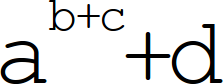
\includegraphics[height=4em]{images/simple.png} \\
\\
\large\( \left\{(\left\{\left\{A \string^ B\right\}\left\{C \string^ D\right\}\right\}/\left\{\left\{\left\{E \string^ F \_ G\right\}+\right\}H\right\})-\right\}I \) \vfill  & 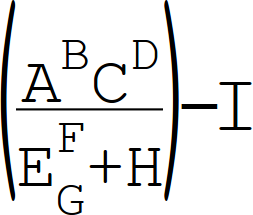
\includegraphics[height=8em]{images/catedra.png} \\
\\
\large\( a \string^ \left\{b \string^ \left\{c \string^ \left\{d \string^ \left\{e \string^ \left\{f \string^ \left\{g \string^ \left\{h \string^ \left\{i \string^ \left\{j \string^ \left\{k \string^ \left\{l\right\}\right\}\right\}\right\}\right\}\right\}\right\}\right\}\right\}\right\}\right\} \) \large\(\_ \left\{n \_ \left\{o \_ \left\{p \_ \left\{q \_ \left\{r \_ \left\{s \_ \left\{t \_ \left\{u \_ \left\{v \_ \left\{w \_ \left\{x\right\}\right\}\right\}\right\}\right\}\right\}\right\}\right\}\right\}\right\}\right\} \) \large\( +yz \) \vfill & 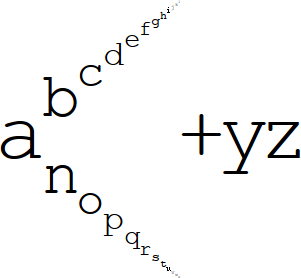
\includegraphics[height=8em]{images/doublemountain.png} \\
\\
\large \( \left\{a \string^ b \_ \left\{c \_ \left\{i \_ \left\{j\right\}\right\}\right\} / \right. \) \( \left. d \string^ \left\{e \string^ \left\{f \string^ \left\{k \string^ \left\{l\right\}\right\}\right\} \_ g\right\} +m+n+o+p \right\}+h \) \vfill & 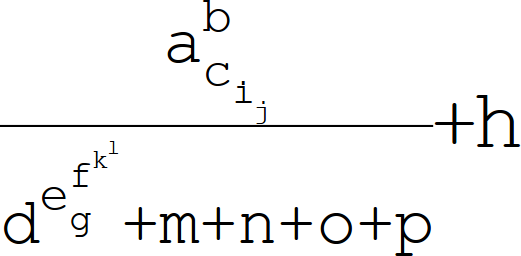
\includegraphics[height=7em]{images/division.png} \\

\\
\large\( (a)+(b \string^ \left\{c \string^ d \_ \left\{e \string^ \left\{f \string^ \left\{g \string^ \left\{h \string^ \left\{i \string^ \left\{j\right\}\right\}\right\}\right\}\right\}\right\}\right\} \_ \) \( \left\{k \_ \left\{l \_ \left\{m \_ \left\{n \_ \left\{o\right\}\right\}\right\}\right\}\right\})+p-q \) \vfill & 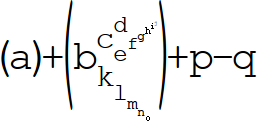
\includegraphics[height=7em]{images/parenmountains.png} \\
\\
\large\(A+\) \((B)\left\{G\string^\left\{(F\string^e\_E/(2))\right\}\right.- \) \(\left.(Q\_\left\{E\_\left\{\left\{5\right\}+E\_\left\{E\_\left\{E\_D\right\}\right\}\right\}\right\}-Y)\right.\) \(\left.+X\string^K\_J/Y\right\}-\left\{(80)/(2)\right\}-\left\{C\string^\left\{G\string^\left\{G\string^\left\{G\right\}\right\}\right\}/5\right\}/(\left\{8+4+7\right\}+5/ee)\string^\left\{-i\right\}\) \vfill & 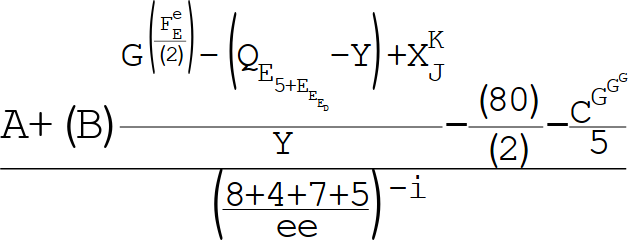
\includegraphics[height=11em]{images/christian.png} \\
\end{tabular}
\end{adjustwidth}

\section{C\'odigo fuente}

\subsection{formula.l}

\begin{lstlisting}[language=C]
%{
#include <stdio.h>
#include "formula.tab.h"
%}

%%

[ \t] ;

"\n" { return T_ENDLINE; }

"(" { return T_OPENPAREN; }
")" { return T_CLOSEPAREN; }
"{" { return T_OPENBRACKET; }
"}" { return T_CLOSEBRACKET; }
"/" { return T_DIV; }
"^" { return T_CARET; }
"_" { return T_UNDER; }

[^^_/{}() \t] { return T_ID; }

%%
\end{lstlisting}

\subsection{formula.y}

\begin{lstlisting}[language=C]
%{
#include <stdio.h>
#include <stdlib.h>
#include <stdbool.h>
#include <string.h>
#include <math.h>
#include <assert.h>

// Operaciones posibles.
enum Operation
{
	Literal,
	Concat,
	Caretunder,
	Parentheses,
	Division
};

// El tamano de una expresion.
struct Size
{
	double x; // Ancho
	double ny, my; // Altura baja y altura alta.
};

// Una expresion.
struct Expression
{
	struct Expression *left, *right; // Expresiones hijos. Pueden ser NULL.
	char c; // Caracter que representa, si es de tipo Literal.

	enum Operation t; // Tipo de esta expresion.
	struct Size d; // Tamano de la expresion. Asignada por sizeExpression.
};

extern int yylex();
extern int yyparse();
extern char* yytext;

#define YYSTYPE_IS_DECLARED
typedef struct Expression *YYSTYPE;

YYSTYPE buildToken(char);
YYSTYPE buildExpression(enum Operation, YYSTYPE, YYSTYPE);
void sizeExpression(YYSTYPE);
void printExpression(YYSTYPE);
void printSVG(YYSTYPE);

void yyerror(const char *);
%}

%token T_DIV
%token T_CARET T_UNDER
%token T_OPENPAREN T_CLOSEPAREN T_OPENBRACKET T_CLOSEBRACKET
%token T_ID
%token T_ENDLINE

%start init

%%

init: e T_ENDLINE { sizeExpression($$); printSVG($$); }

e:	  f T_DIV e { $$ = buildExpression(Division, $1, $3); }
	| f

f:	  g f { $$ = buildExpression(Concat, $1, $2); }
	| g

g:	  h T_CARET h { $$ = buildExpression(Concat, $1, buildExpression(Caretunder, $3, NULL)); }
	| h T_UNDER h { $$ = buildExpression(Concat, $1, buildExpression(Caretunder, NULL, $3)); }
	| h T_CARET h T_UNDER h { $$ = buildExpression(Concat, $1, buildExpression(Caretunder, $3, $5)); }
	| h T_UNDER h T_CARET h { $$ = buildExpression(Concat, $1, buildExpression(Caretunder, $5, $3)); }
	| h

h:	  T_OPENPAREN e T_CLOSEPAREN { $$ = buildExpression(Parentheses, $2, NULL); }
	| T_OPENBRACKET e T_CLOSEBRACKET { $$ = $2; }
	| T_ID { $$ = buildToken(yytext[0]); }

%%

bool debug = false;

// Devuelve un nodo hoja, que tiene cierto caracter.
YYSTYPE buildToken(char c)
{
	YYSTYPE r = malloc(sizeof (struct Expression));
	r->c = c;
	r->t = Literal;
	r->left = r->right = NULL;

	return r;
}

// Devuelve una expresion representada por cierta operacion, y con dos hijos.
YYSTYPE buildExpression(enum Operation op, YYSTYPE left, YYSTYPE right)
{
	YYSTYPE r = malloc(sizeof (struct Expression));
	r->c = '\0';
	r->t = op;
	r->left = left;
	r->right = right;

	return r;
}

// Devuelve el tamano de un nodo que representa cierta operacion, y tiene
// ciertos hijos. Los hijos ya deben tener su tamano calculado.
struct Size getSizes(enum Operation t, YYSTYPE left, YYSTYPE right)
{
	switch (t)
	{
		case Literal:
			return (struct Size) {.x = 7, .ny = -6, .my = 0};

		case Concat:
			return (struct Size) {.x = left->d.x + right->d.x, .ny = fmin(left->d.ny, right->d.ny), .my = fmax(left->d.my, right->d.my)};

		case Caretunder:
		{
			struct Size r = {0, 0};
			if (left)
			{
				r.x = fmax(r.x, left->d.x * .75);
				r.ny = left->d.ny * .75 - 6;
			}
			if (right)
			{
				r.x = fmax(r.x, right->d.x * .75);
				r.my = right->d.my * .75 + 5;
			}
			return r;
		}

		case Parentheses:
			return (struct Size) {.x = left->d.x + 11, .ny = left->d.ny - 2, .my = left->d.my + 4};

		case Division:
			return (struct Size) {.x = fmax(left->d.x, right->d.x) * .8, .ny = left->d.ny * .8 - left->d.my - 4, .my = right->d.my * .8 - right->d.ny - 0.5};
	}

	fprintf(stderr, "Invalid operation under calculate: %d\n", t);
	exit(1);
}

// Calcula el tamano de los hijos de un nodo, y usa estos valores para
// asignarle un tamano a este nodo.
void sizeExpression(YYSTYPE q)
{
	if (q == NULL)
		return;

	sizeExpression(q->left);
	sizeExpression(q->right);

	q->d = getSizes(q->t, q->left, q->right);
}

// Imprime un nodo con cierta transformacion en x, y, y tamano.
void transformExpression(YYSTYPE q, double dx, double dy, double ds)
{
	if (q == NULL)
		return;

	printf("<g transform=\"translate(%lf %lf) scale(%lf)\">\n", dx, dy, ds);
	printExpression(q);
	printf("</g>\n");
}

// Imprime un nodo y sus hijos.
void printExpression(YYSTYPE q)
{
	if (q == NULL)
		return;

	switch (q->t)
	{
		case Literal:
			printf("<text>%c</text>\n", q->c);
			break;

		case Concat:
			printExpression(q->left);
			transformExpression(q->right, q->left->d.x, 0, 1);
			break;

		case Caretunder:
			transformExpression(q->left, 0, -6, .75);
			transformExpression(q->right, 0, 5, .75);
			break;

		case Parentheses:
		{
			double height = (q->d.my - q->d.ny) / 10;
			printf("<text transform=\"scale(1 %lf) translate(0 %lf)\">(</text>\n", height, height / 2);
			transformExpression(q->left, 6, 0, 1);
			printf("<text transform=\"scale(1 %lf) translate(%lf %lf)\">)</text>\n", height, q->left->d.x + 5, height / 2);
			break;
		}

		case Division:
			transformExpression(q->left, (q->d.x - q->left->d.x * .8) / 2, -q->left->d.my * .8 - 4, .8);
			printf("<line stroke-width=\"0.3\" stroke=\"black\" x1=\"0\" x2=\"%lf\" y1=\"-3\" y2=\"-3\" />\n", q->d.x);
			transformExpression(q->right, (q->d.x - q->right->d.x * .8) / 2, -q->right->d.ny * .8 - 0.5, .8);
			break;

		default:
			fprintf(stderr, "Invalid operation under print: %d\n", q->t);
			exit(1);
	}

	if (debug && q->t != Concat)
	{
		const char *colors[] = {"black", "red", "blue", "green", "purple"};

		printf("<line stroke-width=\".1\" stroke=\"%s\" x1=\"0\" x2=\"%lf\" y1=\"%lf\" y2=\"%lf\" />\n", colors[q->t], q->d.x, q->d.ny, q->d.ny);
		printf("<line stroke-width=\".1\" stroke=\"%s\" x1=\"0\" x2=\"%lf\" y1=\"%lf\" y2=\"%lf\" />\n", colors[q->t], q->d.x, q->d.my, q->d.my);
	}
}

// Imprime el SVG correspondiente a un arbol sintactico con raiz q. El tamano
// de q y sus hijos ya debe estar calculado.
void printSVG(YYSTYPE q)
{
	puts("<?xml version=\"1.0\" standalone=\"no\"?>");
	puts("<!DOCTYPE svg PUBLIC \"-//W3C//DTD SVG 1.1//EN\" \"http://www.w3.org/Graphics/SVG/1.1/DTD/svg11.dtd\">");
	puts("<svg xmlns=\"http://www.w3.org/2000/svg\" version=\"1.1\">");

	printf("<g transform=\"translate(50, %lf) scale(7)\" font-family=\"monospace\">\n", 300 - q->d.ny);

	printExpression(q);

	puts("</g>");
	puts("</svg>");
}

// Indica que hubo un error en el parseo.
void yyerror(const char* s)
{
	fprintf(stderr, "Parse error: %s\n", s);
	exit(1);
}

// Parsea la entrada, y activa el flag de debug si ese es el argumento.
int main(int argc, char *argv[])
{
	if (argc > 1 && !strcmp(argv[1], "--debug"))
		debug = true;

	yyparse();
}
\end{lstlisting}


\end{document}
